\documentclass[a4paper]{article}
\usepackage{graphicx}
\usepackage{twocolpceurws}
\usepackage{float}
\usepackage{hyperref}

\title{Using Refactoring Techniques to Reduce Duplication in Object-Oriented Programming Languages\\- Work in Progress -}

\author{
Simon Baars \\ University of Amsterdam\\
                Puiflijk, Netherlands \\ simon.mailadres@gmail.com
\and
Ana Oprescu \\ University of Amsterdam\\
                Amsterdam, Netherlands \\ A.M.Oprescu@uva.nl
}

\institution{}


\begin{document}
\maketitle
% In this paper I talk about clone instances and clone classes. Should I explain those concepts first?

\begin{abstract}
Duplication in source code can have a major negative impact on the maintainability of source code. There are several techniques that can be used in order to merge clones, reduce duplication and potentially also reduce the total volume of a software system. In this study, we look into the opportunities to aid in the process of refactoring these duplication problems for object-oriented programming languages. Measurements that have been conducted so far have indicated that more than half of the duplication in code is related to each other through inheritance, making it easier to refactor these clones in a clean way. More measurements will be conducted to get a detailed overview of in what contexts clones occur, and what this means for the refactoring processes of these clones. As a desired output, we strive to construct a model that automatically applies refactorings for a large part of the detected duplication problems and implement this model for the Java programming language.
\end{abstract}


\section{Introduction}
Duplication in source code is often seen as one of the most harmful types of technical debt. In Martin Fowler's ``Refactoring'' book \cite{fowler1999refactoring}, he exclaims that \textit{``Number one in the stink parade is duplicated code. If you see the same code structure in more than one place, you can be sure that your program will be better if you find a way to unify them.''}. In this research, we take a look at the challenges and opportunities in automatically refactoring duplicated code, also known as ``code clones''. The main goal is to improve the maintainability of the refactored code.

Refactoring is used to improve quality related attributes of a codebase (maintainability, performance, etc.) without changing the functionality. There are many methods that have been introduced to help with the process of refactoring \cite{fowler1999refactoring, wake2004refactoring}, that are integrated into most modern IDE's. However, most of these methods still require manual assessment of where and when to apply them. Because of this, refactoring takes up a signification portion of the development process \cite{lientz1978characteristics, mens2004survey}, or does not happen at all \cite{mens2003refactoring}. For a large part, refactoring requires domain knowledge to do it right. However, there are also refactoring opportunities that are rather trivial and repetitive to execute. In this research we will look at to what extend code clones can be automatically refactored.

Code clones can be found anywhere in a codebase. The location of a clone in the code has an impact on how it has to be refactored. Because of this, we will first look at where clones can be found. Using this information we can determine in which locations clones are found the most, on basis of which the refactoring will be prioritized. Apart from that, we will look at different types of clones. A duplicate part in a codebase does not always have to be an exact match with another part to be called a clone. We will look at the definitions of different types of clones and what the opportunities are to refactor duplicate parts of code if it's not an exact match. All of these measurements are performed on a large corpus of open source projects. We lay the main focus on the Java programming language as refactoring opportunities feature paradigm and programming language dependent aspects \cite{choi2011extracting}. However, most practises featured in this research will also be applicable with other object-oriented languages, like C\#.

\subsection{Background}
As code clones are seen as one of the most harmful types of technical debt, they have been studied very extensively. A survey by Roy et al \cite{roy2007survey} states definitions for various important concepts in code clone research. In this survey he mentions the concept ``clone pair'', which is \textit{a set of two code portions/fragments which are identical or similar to each other}. Furthermore, he defined ``clone class'' as \textit{the union of all clone pairs}. Apart from this, we use the definition ``clone instance'', which is a single code portion/fragment that is part of either a clone pair or clone class.

A tool called DCRA (Duplicated Code Refactoring Advisor) looks into refactoring opportunities for clone pairs \cite{fontana2012duplicated}. This tool chooses to only focus on refactoring clone pairs because they argue that \textit{clone pairs are much easier to manage when considered singularly.} As intermidiate steps the authors measure a corpus of Java systems for some clone-related properties of the systems, like the relation (in terms of inheritance) between code fragments in a clone pair.

Another tool called Aries \cite{higo2004aries, higo2008metric} focuses on the detection of refactoring oriented clones. In this paper the authors describe a few variables by which a clone can be assessed for refactoring suitability. This tool looks however only at the possibility to merge clones, rather than whether clones should be merged. Also, this tool only suggests refactorings, and does not apply them.

There are many other publications that look into code clone refactoring \cite{alwaqfi2017refactoring, chen2018clone, koni2001scenario}. However, none of the publications describing a refactoring tool have published their source code or application for refactoring support. Also, these publications/tools are limited to suggesting refactoring opportunities for clones found, rather than actually applying refactorings where suitable. Furthermore, all of these tools only support a subset of all harmful clones that are found. Furthermore, all published approaches have limitations, for instance false positives when detecting clones \cite{chen2018clone} or being limited to clone pairs \cite{higo2008metric}.

For this research, we strive to improve upon the current state-of-the-art in clone refactoring by building a clone refactoring tool that applies refactorings to a large percentage of clones found. The design decisions for this tool will be made on basis of data gathered from a large corpus of software systems. The tool will be developed on GitHub and stored in the Software Heritage \cite{di2017software} archives to ensure long term preservation. This way we strive to make the problem of duplication in source code easier to deal with.

\section{Clone Detection}
As duplication in source code is a serious problem in many software systems, there are a lot of researches that look into code clones. Many tools have been proposed to detect various types of code clones. Two surveys of modern clone detection tools \cite{sheneamer2016survey, svajlenko2014evaluating} together show an overview of the most-popular clone detection tools up until 2016. To be able to refactor detected clones, it is useful to have the ability to rewrite the AST. We considered a set of clone detection tools for their ability to support the refactoring process automatically. None of the tools we consider seemed completely fit for this purpose, so we decided to implement our own clone detection tool: CloneRefactor\footnote{CloneRefactor (WIP) is available on GitHub: \url{https://github.com/SimonBaars/CloneRefactor}}.

\subsection{CloneRefactor}
A 2016 survey by Gautam \cite{gautam2016various} focuses more on various techniques for clone detection. For our tool we decided to combine AST and Graph based approaches for clone detection, similar to Scorpio (which is a clone detection tool that's part of TinyPDG: a library for building intraprocedural program dependency graphs for Java programs). We decided to base our tool on the JavaParser library \cite{tomassetti2017javaparser}, as it supports rewriting the AST back to Java code and is useable with all modern Java versions (Java 1-12). We collect each statement and declaration and compare those to find duplicates. This way we build a graph of each statement/declaration linking to each subsequent statement/declaration (horizontally) and linking to each of it's duplicates (verically). This is displayed in figure \ref{fig:clonerefactor}.

\begin{figure}[H]
  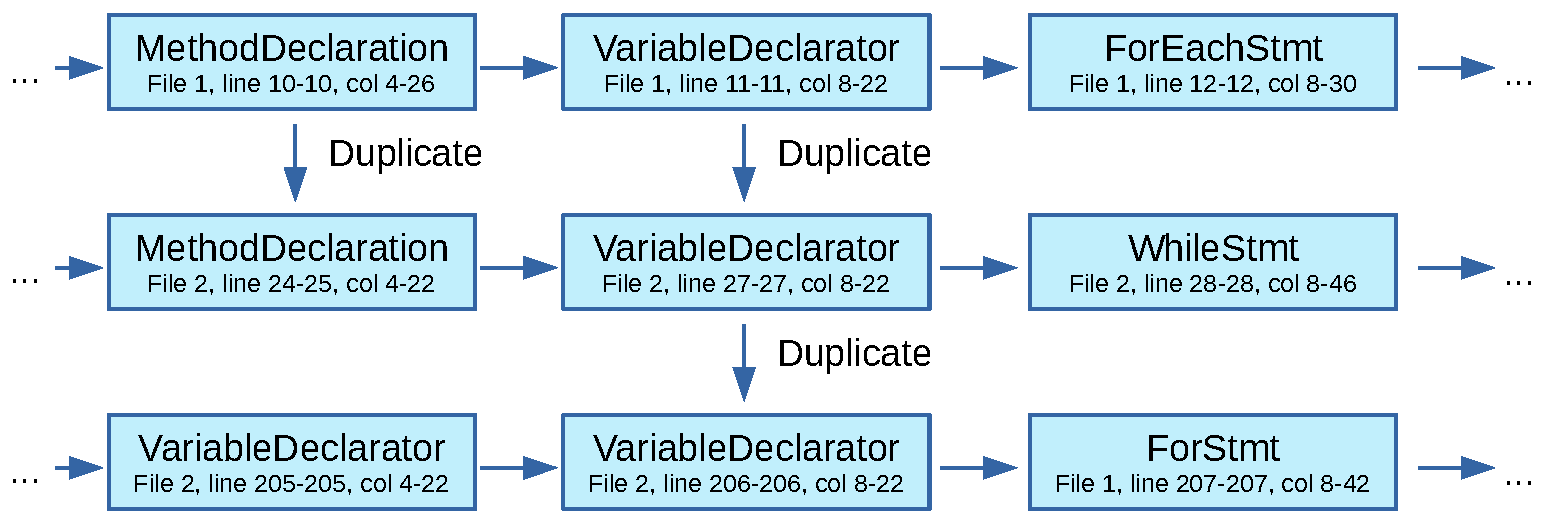
\includegraphics[width=1\columnwidth]{img/CodeGraph}
  \caption{Abstract figure of the graph representation built by CloneRefactor}
  \label{fig:clonerefactor}
\end{figure}

\subsection{Thresholds}
CloneRefactor works on basis of three thresholds for finding clones:
\begin{enumerate}
  \item \textbf{Number of statements/declarations:} The amount of statements/declarations that should be equal/similar for it to be considered a clone.
  \item \textbf{Number of tokens:} The amount of tokens (excluding whitespace, end-of-line terminators and comments) that should be equal/similar for it to be considered a clone.
  \item \textbf{Number of lines:} The minimum amount of lines (excluding lines that do not contain any tokens, for tokens same exclusions apply) that should be equal/similar for it to be considered a clone.
\end{enumerate}
Of course, if we put any of these thresholds to zero it won't be taken into account anymore, so not all thresholds have to be used at all times. We consider ``number of lines'' to be the least important, as it highly depends on the programmer of the codebase (and we do not want this kind of dependence!). On basis of manual assessment, we have determined that setting the ``number of statements/declarations'' to 6 ensures that most non-harmful clones are filtered out. On the downside, this also filters out some harmful antipatterns, for instance if a cloned line has many tokens we might want to consider a clone if it spans less than 6 statements (as cloned line with many tokens is more harmful than one with few).

For the measurements in the next chapter we have chosen to apply the following thresholds:
\begin{itemize}
  \item \textbf{Number of statements/declarations:} 6
  \item \textbf{Number of tokens:} 10
  \item \textbf{Number of lines:} 6
\end{itemize}

\section{Code Clone Context}
To be able to refactor code clones, it is very important to consider the context of the clone. We define the following aspects of the clone as its context:
\begin{enumerate}
  \item The relation of clone instances among each other (for example: two clone instances in a clone class are part of the same object).
  \item Where a clone instance occurs in the code (for instance: a method-level clone is a clone instance that is (a part of) a single method).
  \item The contents of a clone instance (for instance: the clone instance consists of a one method declaration, a foreach statement and two variable declarations).
\end{enumerate}
Everything in the context of a clone has a big impact on how it has to be refactored. For this study we performed measurements on the context of clones in a large corpus of open source projects.

\subsection{The corpus}
For our measurements we use a large corpus of open source projects \cite{githubCorpus2013}\footnote{The corpus can be downloaded from the following URL: \url{http://groups.inf.ed.ac.uk/cup/javaGithub/java_projects.tar.gz}}. This corpus has been assembled to contain relatively higher quality projects (by filtering by forks). Also, any duplicate projects were removed from this corpus. This results in a variaty of Java projects that reflect the quality of average open source Java systems and are useful to perform measurements on.

We then filtered the corpus further to make sure we are not including any test classes or generated classes. Many Java/Maven projects use a structure where they separate the application and it's tests in the different folders (``/src/main/java'' and ``/src/test/java'' respectively). Because of this, we chose to only use projects from the corpus which use this structure (and had at least a ``/src/main/java'' folder). To limit the execution time of the script, we also decided to limit the maximum amount of source files in a single project to 1.000 (projects with more source files were not considered, which filtered only 5 extra projects out of the corpus). Of the 14.436 projects in the corpus over 3.848 remained, which is plenty for our purposes. The script to filter the corpus in included in our GitHub repository \footnote{The script we use to filter the corpus: \url{https://github.com/SimonBaars/CloneRefactor/blob/MeasurementsVersion1/src/main/java/com/simonbaars/clonerefactor/scripts/PrepareProjectsFolder.java}}.

Running our clone detection script, CloneRefactor, over this corpus gives the results displayed in table \ref{table:general}.

\begin{table}[H]
  \begin{center}
  \caption{CloneRefactor results for Java projects corpus \cite{githubCorpus2013}.} \label{table:general}
  \bigskip
\begin{tabular}{|l|l|}
\hline
Amount of projects                                                                                      & 3.848      \\ \hline
Amount of lines                                                                                         & 8.284.140  \\ \hline
\begin{tabular}[c]{@{}l@{}}Amount of lines (excluding\\ whitespace, comments, etc.)\end{tabular}        & 8.163.429  \\ \hline
Amount of statements/declarations                                                                       & 6.863.725  \\ \hline
Amount of tokens                                                                                        & 66.964.270 \\ \hline
Amount of lines cloned                                                                                  & 1.341.094  \\ \hline
\begin{tabular}[c]{@{}l@{}}Amount of lines cloned (excluding\\ whitespace, comments, etc.)\end{tabular} & 815.799    \\ \hline
\begin{tabular}[c]{@{}l@{}}Amount of statements/declarations\\ cloned\end{tabular}                      & 747.993    \\ \hline
Amount of tokens cloned                                                                                 & 9.800.819  \\ \hline
Amount of clone classes                                                                                 & 34.367     \\ \hline
\end{tabular}
\end{center}
\end{table}

\subsection{Relations Between Clone Instances}
When merging code clones in object-oriented languages, it is very important to consider the relation between clone instances.

\subsubsection{Categorizing Clone Instance Relations}
A paper by Fontana et al \cite{fontana2015duplicated} performs measurements on 50 open source projects on the relation of clones to each other. To do this, they first define several categories for the relation between clone instances in object-oriented languages. These categories are as follows:
\begin{enumerate}
  \item \textbf{Same method}: All instances of the clone class are in the same method.
  \item \textbf{Same class}: All instances of the clone class are in the same class.
  \item \textbf{Superclass}: All instances of the clone class are children and parents of each other.
  \item \textbf{Ancestor class}: All instances of the clone class are superclasses except for the direct superclass.
  \item \textbf{Sibling class}: All instances of the clone class have the same parent class.
  \item \textbf{First cousin class}: All instances of the clone class have the same grandparent class.
\item \textbf{Common hierarchy class}: All instances of the clone class belong to the same hierarchy, but do not belong to any of the other categories.
\item \textbf{Same external superclass}: All instances of the clone class have the same superclass, but this superclass is not included in the project but part of a library.
\item \textbf{Unrelated class}: There is at least one instance in the clone class that is not in the same hierarchy.
\end{enumerate}
Please note that no of these categories allow external classes (except for ``same external superclass''). So if two clone instances are related through external classes but do not share a common external superclass, it will be flagged as ``unrelated''. The main reason for this is that it is (often) not possible to refactor to external classes.

The ranking of the previous list of categories also matters, as it shows the different levels in which clones were assessed. For instance, if two clone instances of a clone class belong to the ``same method'' category but the third belongs to the ``same class'', we will always chose the item lowest on the list.

\subsubsection{Our measurements}
We have recreated table 3 of Fontana et al \cite{fontana2015duplicated}, but with the following differences in our setup:
\begin{itemize}
  \item We consider clone classes rather than clone pairs.
\item We use different thresholds regarding when a clone should be considered.
\item We seek by statement/declaration rather than SLOC.
\item We test a broader range of projects (they use a set of 50 relatively large projects, we use a large corpus that was assembled by a machine learning algorithm testing java projects on GitHub for quality, which contains projects of all sizes and with differing code quality).
\end{itemize}

Table \ref{table:relations} contains our results regarding the relations between clone instances.

\begin{table}[H]
  \begin{center}
  \caption{Clone relations} \label{table:relations}
  \bigskip
\begin{tabular}{|l|l|l|} \hline
\textbf{Relation}  & \textbf{Amount} & \textbf{Percentage} \\ \hline
Unrelated          & 13.529           & 39,37               \\ \hline
Same Class          & 8.341            & 24,28               \\ \hline
Sibling            & 5.978            & 17,40               \\ \hline
Same Method         & 2.456            & 7,15                \\ \hline
External Superclass & 2.402            & 6,99                \\ \hline
First Cousin        & 695             & 2,02                \\ \hline
Superclass         & 489             & 1,42                \\ \hline
Common Hierarchy    & 442             & 1,29                \\ \hline
Ancestor           & 28              & 0,08               \\ \hline
\end{tabular}
\end{center}
\end{table}

Comparing it to the results of Fontana et al \cite{fontana2015duplicated}, we find way more unrelated clones. This might be due to the fact that we consider clone classes rather than clone pairs, and mark the clone class ``Unrelated'' even if just one of the clone instances is outside a hierarchy. It could also be that the corpus which we use, as it has generally smaller projects, use more classes from outside the project (which are marked UNRELATED if they do not have a common external superclass). On the second place, we have the ``Same Class'' clones. On the third place come the ``Sibling'' clones.

\subsection{Clone instance location}
After mapping the relations between individual clones, we looked at the location of individual clone instances. A paper by Lozano et al \cite{lozano2007evaluating} discusses the harmfulness of cloning. In this paper the author argues that 98\% are produced at method-level. However, this claim is based on a very small dataset and a questionable way of measurement. We validated this claim over our corpus. For this, we chose the following categories:
\begin{enumerate}
  \item \textbf{Method/Constructor Level:} A clone instance that does not exceed the boundaries of a single method or constructor (optionally including the declaration of the method or constructor itself).
  \item \textbf{Class Level:} A clone instance in a class, that exceeds the boundaries of a single method or contains something else in the class (like field declarations, other methods, etc.).
  \item \textbf{Interface Level:} A clone that is (a part of) an interface.
  \item \textbf{Enumeration Level:} A clone that is (a part of) an enumeration.
\end{enumerate}

A paper by Lozano et al \cite{lozano2007evaluating} discusses the harmfulness of cloning. In this paper the author argues that 98\% are produced at method-level. However, their source for this information, uses a very questionable techique of measuring (human copy-paste behaviour with a small sample-size). We set out to test this for ourselves on the corpus of Java projects which we used for all our measurements. The results for the clone instance locations are shown in table \ref{table:locations}.

\begin{table}[H]
  \begin{center}
  \caption{Clone instance locations} \label{table:locations}
  \bigskip
\begin{tabular}{|l|l|l|}
\hline
\textbf{Location}  & \textbf{Amount}  & \textbf{Percentage} \\ \hline
Method Level       & 19.818           & 57,68               \\ \hline
Class Level        & 13.259           & 38,59               \\ \hline
Constructor Level  & 1.099            & 3,20                \\ \hline
Interface Level    & 110              & 0,32                \\ \hline
Enum Level         & 74               & 0,22                \\ \hline
\end{tabular}
\end{center}
\end{table}

From these results we can see, somewhat surprisingly, that the claim of 98\% of clones being produced at method-level is nowhere near correct. In fact, around 58\% of the clones are produced at method-level. About 39\% of clones either span several methods/constructors or contain something like a field declaration. Another 3\% of the clones is found in contructors. The amount of clones found in interfaces and enumerations is very low.

\subsection{Clone instance contents}
Finally, we looked at the contents of individual clone instances: what kind of declarations and statements do they span. We selected the following categories to be relevant for refactoring:
\begin{enumerate}
  \item \textbf{Full Method/Class/Interface/Enumeration:} A clone that spans a full class, method, constructor, interface or enumeration, including its declaration.
  \item \textbf{Partial Method/Constructor:} A clone that spans a method partially, optionally including its declaration.
  \item \textbf{Several Methods:} A clone that spans over two or more methods, either fully or partially, but does not span anything but methods (so not fields or anything in between).
  \item \textbf{Only Fields:} A clone that spans only global variables.
  \item \textbf{Includes Fields/Constructor:} A clone that spans a combination of fields and other things, like methods.
  \item \textbf{Method/Class/Interface/Enumeration Declaration:} A clone that contains the declaration (usually the first line) of a class, method, interface or enumeration.
  \item \textbf{Other:} Anything that does not match with above stated categories.
\end{enumerate}

The results for these categories are displayed are displayed in table \ref{table:contents}.

\begin{table}[H]
  \begin{center}
  \caption{Clone instance contents} \label{table:contents}
  \bigskip
\begin{tabular}{|l|l|l|}
  \hline
  \textbf{Contents}                                                        & \textbf{Amount} & \textbf{Percentage} \\ \hline
  Partial Method                                                           & 19.264          & 56,07               \\ \hline
  Several Methods                                                          & 9.076           & 26,41               \\ \hline
  Includes Constructor                                                     & 1.528           & 4,45                \\ \hline
  Includes Field                                                           & 1.149           & 3,34                \\ \hline
  Partial Constructor                                                      & 1.098           & 3,20                \\ \hline
  Only Fields                                                              & 565             & 1,64                \\ \hline
  Full Method                                                              & 554             & 1,61                \\ \hline
  \begin{tabular}[c]{@{}l@{}}Includes Class\\ Declaration\end{tabular}     & 445             & 1,30                \\ \hline
  Other                                                                    & 369             & 1,07                \\ \hline
  Full Class                                                               & 192             & 0,56                \\ \hline
  \begin{tabular}[c]{@{}l@{}}Includes Enum\\ Constant\end{tabular}         & 52              & 0,15                \\ \hline
  \begin{tabular}[c]{@{}l@{}}Includes Enum\\ Declaration\end{tabular}      & 47              & 0,14                \\ \hline
  \begin{tabular}[c]{@{}l@{}}Includes Interface\\ Declaration\end{tabular} & 10              & 0,03                \\ \hline
  Full Interface                                                           & 6               & 0,02                \\ \hline
  Full Enumeration                                                         & 4               & 0,01                \\ \hline
\end{tabular}
\end{center}
\end{table}

Unsurprisingly, most clones span a part of a method. Just 1.6\% of the methods are cloned fully. More than a quarter of the clones spans over several methods, which is surprising. Simply extracting methods won't work in a case where a clone spans over several methods. About 4.5\% of clones include a constructor. About 3.3\% of clones include a global variable defined in a class.

\section{Redefining type-2 and type-3 clones}
In a 2007 survey by Roy et al \cite{roy2007survey} he defined four types of clones:

\textbf{Type I:} Identical code fragments except for variations in whitespace (may be also variations in layout) and comments.\\
\textbf{Type II:} Structurally/syntactically identical fragments except for variations in identifiers, literals, types, layout and comments.\\
\textbf{Type III:} Copied fragments with further modifications. Statements can be changed, added or removed in addition to variations in identifiers, literals, types, layout and comments.\\
\textbf{Type IV:} Two or more code fragments that perform the same computation but implemented through different syntactic variants.

\section{Merging duplicate code through refactoring}
Now we have mapped the contexts in which clones occur, we can start looking at refactoring opportunities. Regarding refactoring, we separate clones in two categories: easy and difficult refactoring opportunities. Easy refactoring opportunities are clones that can easily be automatically refactored. Examples of these opportunities are fully cloned methods or a set of fully cloned statements. According to the relation between the clone instances, we can propose a refactoring automatically.

However, not always can a clone easily be merged. Sometimes a clone spans a statement partially (like a for-loop of which only it's declaration and a part of the body is cloned). Merging the clones can be harder in such instances. Also, cloned code can contain a complex control structure, like labels, return, break, continue, etc. In such instances, more conditions apply do be able to conduct a refactoring, if advisable at all.

%TODO: Show measurements

\section{Threats to validity}
We noticed that, when measuring over a corpus of this size, the thresholds that we use for the clone detection have a big impact on the results. There does not seem to be one golden set of thresholds, some thresholds work in some situations but fail in others. We have chosen thresholds that, according to our manual assessment, seemed optimal. However, by using these, we definitely miss some harmful clones.

\section{Conclusion and next steps}
Next step: build the model to automatically refactor!

%TODO: Expand conclusion

\subsubsection{Acknowledgements}
We would like to thank the Software Improvement Group (SIG) for their continuous support in this project.




\bibliographystyle{alpha}
\bibliography{res}

\end{document}
